% File SDSS2020_SampleExtendedAbstract.tex
\documentclass[10pt]{article}\usepackage[]{graphicx}\usepackage[]{color}
% maxwidth is the original width if it is less than linewidth
% otherwise use linewidth (to make sure the graphics do not exceed the margin)
\makeatletter
\def\maxwidth{ %
  \ifdim\Gin@nat@width>\linewidth
    \linewidth
  \else
    \Gin@nat@width
  \fi
}
\makeatother

\definecolor{fgcolor}{rgb}{0.345, 0.345, 0.345}
\newcommand{\hlnum}[1]{\textcolor[rgb]{0.686,0.059,0.569}{#1}}%
\newcommand{\hlstr}[1]{\textcolor[rgb]{0.192,0.494,0.8}{#1}}%
\newcommand{\hlcom}[1]{\textcolor[rgb]{0.678,0.584,0.686}{\textit{#1}}}%
\newcommand{\hlopt}[1]{\textcolor[rgb]{0,0,0}{#1}}%
\newcommand{\hlstd}[1]{\textcolor[rgb]{0.345,0.345,0.345}{#1}}%
\newcommand{\hlkwa}[1]{\textcolor[rgb]{0.161,0.373,0.58}{\textbf{#1}}}%
\newcommand{\hlkwb}[1]{\textcolor[rgb]{0.69,0.353,0.396}{#1}}%
\newcommand{\hlkwc}[1]{\textcolor[rgb]{0.333,0.667,0.333}{#1}}%
\newcommand{\hlkwd}[1]{\textcolor[rgb]{0.737,0.353,0.396}{\textbf{#1}}}%
\let\hlipl\hlkwb

\usepackage{framed}
\makeatletter
\newenvironment{kframe}{%
 \def\at@end@of@kframe{}%
 \ifinner\ifhmode%
  \def\at@end@of@kframe{\end{minipage}}%
  \begin{minipage}{\columnwidth}%
 \fi\fi%
 \def\FrameCommand##1{\hskip\@totalleftmargin \hskip-\fboxsep
 \colorbox{shadecolor}{##1}\hskip-\fboxsep
     % There is no \\@totalrightmargin, so:
     \hskip-\linewidth \hskip-\@totalleftmargin \hskip\columnwidth}%
 \MakeFramed {\advance\hsize-\width
   \@totalleftmargin\z@ \linewidth\hsize
   \@setminipage}}%
 {\par\unskip\endMakeFramed%
 \at@end@of@kframe}
\makeatother

\definecolor{shadecolor}{rgb}{.97, .97, .97}
\definecolor{messagecolor}{rgb}{0, 0, 0}
\definecolor{warningcolor}{rgb}{1, 0, 1}
\definecolor{errorcolor}{rgb}{1, 0, 0}
\newenvironment{knitrout}{}{} % an empty environment to be redefined in TeX

\usepackage{alltt}
\usepackage{newtxtext, newtxmath, times}
\usepackage{sdss2020} % Uses Times Roman font (either newtx or times package)
\usepackage{url}
\usepackage{latexsym}
\usepackage{amsmath, amsfonts}
\usepackage{algorithm, algorithmic}  
\usepackage{graphicx}
\usepackage[dvipsnames]{xcolor} % colors

% Commands for editing
\newcommand{\db}[1]{{\textcolor{orange}{#1}}}
\newcommand{\svp}[1]{{\textcolor{blue}{#1}}}

%\title{Symposium on Data Science and Statistics (SDSS 2022) \\
%Submission and Formatting Instructions for Extended Abstracts}

\title{Exploring Rural Shrink Smart Through Guided Discovery Dashboards}

\author{
  Denise Bradford \\
  University of Nebraska - Lincoln \\
  Lincoln, Nebraska \\
  {\tt denise.bradford@huskers.unl.edu} \\\And
  Susan VanderPlas \\
  University of Nebraska - Lincoln \\
  Lincoln, Nebraska \\
  {\tt susan.vanderplas@unl.edu} \\}
  

\date{}
\IfFileExists{upquote.sty}{\usepackage{upquote}}{}
\begin{document}




\maketitle
\begin{abstract}
Many small and rural places are shrinking. Interactive dashboards are the most common use cases for data visualization and context for exploratory data tools. In our paper, we will explore the specific scope of how dashboards are used in small and rural area to empower novice analysts to make data-driven decisions. Our framework will suggest a number of research directions to better support small and rural places from shrinking using an interactive dashboard design, implementation and use for the every day analyst. 
\end{abstract}

{\bf Keywords:} Interactive Dashboards, Exploratory Data Analysis (EDA), Guided Discovery

\section{Research Problem}
With the amount of publicly open-source data, a proliferation of visualization dashboards has increased in nearly every industry \cite{fisher}. A dashboard in its fundamental form, a dashboard supports a way of presenting and making sense of complex data to better enable and support decision making. 

% Stephen Few defines a dashboard as:
% 
% \begin{quotation}% I don't know that we need this... dashboards are very common, so let's focus on the problem and the dashboard as an obvious solution.
% \small A visual display of the most important information needed to achieve one or more objectives, consolidated and arranged on a single screen so the information can be monitored at a glance. \cite{few}
% \end{quotation}

Some communities continue to thrive as they lose population because they adapt\svp{, maintaining quality of life and community services for residents while} investing in the future. % putting sentences on different lines helps with git merges and also makes it easier to figure out where {} match up :)
\svp{This process,} \emph{smart shrinkage}\svp{, is important for rural areas who have experienced shrinking populations for decades.} 
\svp{As small rural towns do not have access to data scientists or even the ability to easily leverage data collected locally to support decisions, our} research team \svp{will provide communities with data about services in small town Iowa in order to assist with} developing strategies to improve quality of life for their residents amid shrinking populations \cite{scc}. \svp{We hope to allow towns to discover their own data and compare to other similar towns, centering decision-making on data in the context of small-town Iowa life. In the process, we will assess our visualizations to determine which strategies for user interface and interactive graphics design are most useful to empower town leaders to make discoveries in publicly available data assembled with a focus on items that impact rural quality of life.}
% Our work focuses on developing and challenges novice analysts in advanced statistical concepts and data visualizations to help make decisions. Specifically, what data can be used to help make decisions, what strategies overcome the challenges of those analysts feel empowered to make data-driven decisions. Our ultimate aim is to help inform Iowa's Rural Shrink Smart communities by using effective dashboards to help those towns build the Quality of Life (QoL) Measures.

\section{Data Description}
\svp{Data collected from \url{data.iowa.gov}} were used to create the SCC dashboard. \svp{Most of these datasets are collected on a town/city or county level, requiring us to carefully join data accounting for differences in spatial resolution.} \svp{\url{data.iowa.gov} contains unique information about residents, including local liquor sales, school building locations, town budgets and expenditures, hospital beds, Medicaid reimbursements, and other details that may provide information about local quality of life.} 
\svp{Using this data, we created a dashboard which allows communities to explore these data and compare and contrast their local community to other communities of similar size and location. In addition to manual comparisons created by the user, we will use statistical clustering methods to identify groups of towns which employ similar strategies to maintain resident quality of life.}

\svp{One of the interesting features of this assembled dataset is that missing data can be missing for multiple reasons: not all state data is complete, but data about certain services may also be missing because towns do not offer that service.}
\svp{Thus, in addition to the usual challenges of working with real-world data that is "messy" in a variety of ways, we also have to contend with missing data that is missing due to the size of the community or the lack of services. This makes both visualization and statistical analysis more complicated.}

\section{Guiding Design Principles}
\svp{An additional challenge is that research on dashboard creation and interactive visualization tends to be very task-specific and not generalizable. That is, it is relatively easy to create a dashboard that works for a particular task, but it is hard to generalize from that process what will work for the next dashboard. With this in mind, we have clearly documented our intentions at each stage of the design and evaluation process, with the goal of gathering some useful information about general dashboard design from the process of creating this specific dashboard.}
\svp{Thus, our initial set of dashboard design principles is as follows: }
\begin{itemize}
\item \svp{The town leaders are the focus audience; thus, the town itself should be the central focus of the app.}
\item \svp{Facilitate comparisons with other towns in order to allow the user to explore other potential solutions to offering services that enhance resident quality of life.}
\item \svp{Present the user with peer comparisons in order to widen the scope of exploration beyond the initial set of obvious peers in the local region.}
\item \svp{Allow for more detailed data and feature requests to improve the dashboard design over time.}
\end{itemize}


\section{Current Progress}
In our research, it is important to use visual orientation of dashboards along with the framework of Guided Discovery Learning (GDL), to make sure that the town analyst has the ability to understand the visual orientation easily as well as guided them to new discovery in the dashboard. 
Stephen Few noted in \italize{Information Dashboard Design: The effective visual communication of data} stated that visual orientation of dashboards is important due to the speed at which perception \cite{few}.

%\begin{quotation}
%\smaller{The visual orientation of dashboards is important due to the speed of perception that’s usually required to monitor information. The faster you must assess what’s going on, the more you should rely on graphical means to display the information. \cite{few} }
%\end{quotation}

Few outlined common mistakes that are made in \italize{Information Dashboard Design}, we will focus on making sure that the following three common mistakes on workplace dashboard development are avoided to make sure that the town analyst have the best path to success:
\begin{itemize}
\item{Choosing inappropriate display media}
\item{Ineffectively highlighting what’s important}
\item{Misusing or overusing color}
\end{itemize}

The outlined list has been used as the guiding light to avoid pitfalls in developing dashboards in the workplace. With the amount of data, our analyst fall into the trap of over ineffectively highlighting what's important along with choosing inappropriate display media and misusing color. This is mostly done, in order to make sure that all of the information is given to the user. This has been a major hurdle when displaying the amount data collected from open-source data for the small towns of Iowa.

%Continue to cite this in the documentation but remove the quotation.

A bit of background on Guided Discovery, which is defined as a environment where "students" are actively discovering knowledge, DeDonno states that we use GDL in our daily lives to make decisions by hints, feedback, and helpful information \cite{dedonno}.
%\begin{quotation}
%\small In our daily lives, we may use a guided discovery process where learning is aided by hints, direction, feedback and other helpful information.  \cite{mayer} \cite{dedonno}
%\end{quotation}

Our current work incorporates the ideas of GDL, in which dashboard design have been used to display a panel with vital statistics making sure that the town's analyst small town is the center of focus. The vital statistics show and highlight the town's financial health, shortest distances from city center to critical resources, such as the fire department, hospital, post offices and public schools. The dashboard includes Quality of Life (QoL) Metrics and the financial health of the small town. Based on the number of variables that are used in making sure that the dashboard is extensive and useful, we implemented the use of parallel coordinate plots to show comparisons between the focus small town with the five similar towns. A parallel (coordinates) plot allowed our town analyst to compare the important features of several individual towns on a set of numeric and categorical variables collected. Historically, parallel coordinate plots have been used in air traffic control to help with collision avoidance algorithms, but has been adapted in the statistical data visualization space with an emphasis on three important considerations: the order, the rotation, and the scaling of the axes. Our coordinate plots, will display variables in categorically and numerically by scaling the data.

To determine the five similar towns, we have implemented unsupervised statistical methods, such as K-means, Principal Component Analysis (PCA), and Hierarchical Clustering, based on distances and services available. We continue to use clustering methods to identify the towns that will be best compare when the analyst interacts with our dashboard. Using GDL, our dashboard make sure that the focus small town is compared to other towns to find ways to improve their town using data-driven decisions. Our research partners have worked with five towns directly, who have agreed to partner with the project to help with identify the best practices that are useful in the Iowa small and rural towns.As a a result, we found out that the small towns do not want to be told what to do but would like to make decisions that are of those who have been apart of the community for generations. Our dashboard will hopefully make sure that the town's analyst are guided in the direction that will help the town's population shrink smart. 

Our dashboard development has become more focus on the GDL such that a continual feedback loop from the town analyst in these five towns has helped provide our team with useful notes that will be adaptive to all of the small towns in Iowa. Our team has captured useful metrics on the use of the product allowing the quantitative and qualitative data collection to better user experience. This can promote challenges in the event of towns feeling "studied" by people in cities outside of their own. 

In Figure 1, our dashboard allows the user to select a town name, which will populate the information in the maps related to necessary services, which include directions and distance to fire department, schools, post offices and hospitals. A table populates in the vital statistics sections that has information about the town's QoL Metrics and financial metrics, followed by a parallel coordinate plot that allows the town to see five towns that are similar based in the most common variables in the towns, such as the distance of fire department. 

\begin{figure}[ht!]
\centering
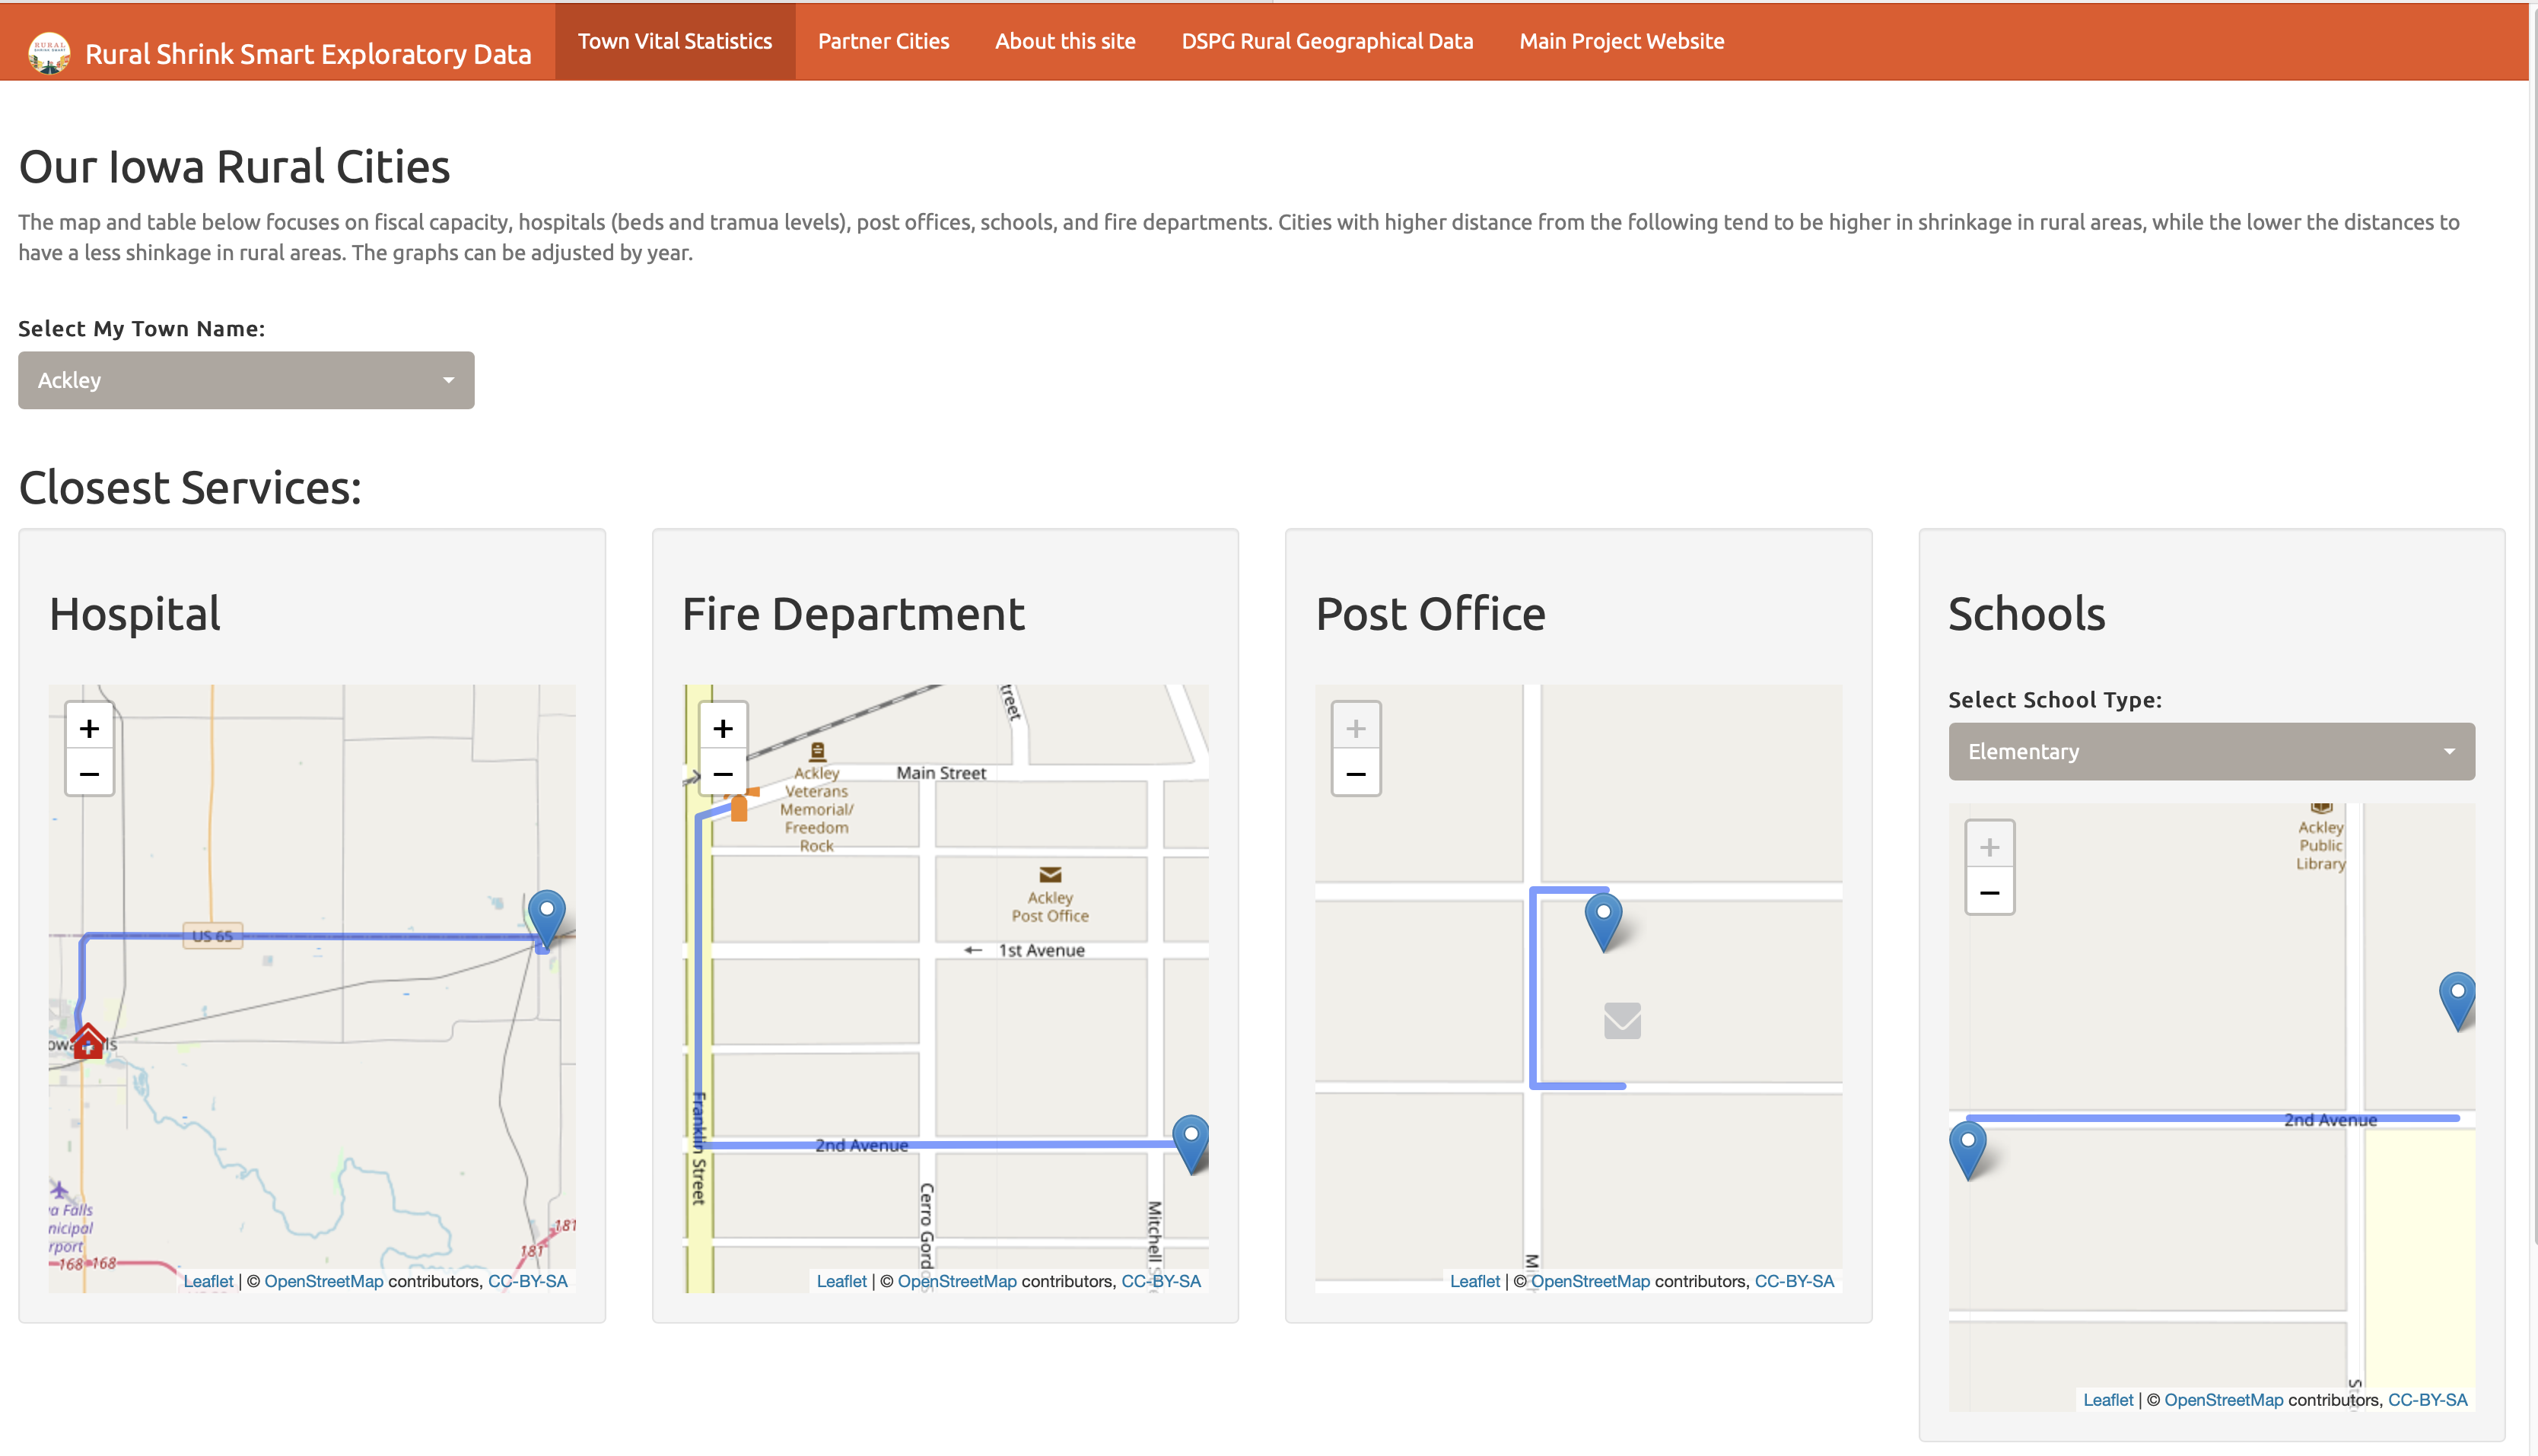
\includegraphics[width=75mm]{SCC_Dashboard.png}
\caption{Rural Smart EDA Dashboard Design}
\end{figure}

%To-Do: Write this in the way that we have done this because by the time that we present this will be done. 
%\subsection{Future Work}

\section{Acknowledgements}
We would like to thank our sponsors and grant provider NSF, LSAMP Inspire Program and Iowa League of Cities. We would like to thank our partners and team members at Iowa State University and University of Nebraska - Lincoln. We would like to thank the State of Iowa for providing Data along with our partners in the Rural Iowa communities.


\bibliographystyle{sdss2020} % Please do not change the bibliography style
\bibliography{SCCAbstract_SDSS2022}

\end{document}
